\documentclass[12pt]{article}
\usepackage[utf8]{inputenc}
\usepackage{listings}
\usepackage{amsmath}
\usepackage{float}
\usepackage{graphicx}
\usepackage{subcaption}

\usepackage[
  a4paper,
  left=20mm,
  right=20mm,
  top=20mm,
  bottom=20mm
]{geometry}

\title{Primo report}
\author{Giacomo Longo (4336477) e Roberta Tassara (4336488)}
\date{14 Novembre 2019}

\begin{document}
% Titolo
\begin{titlepage}
\maketitle
\end{titlepage}

\section{Analisi di regressione}
\subsection{Introduzione}
Il primo caso che analizzeremo riguarda la realizzazione di una stima mediante un approssimatore universale
$$
  h(x) = \sum_{i=0}^{p} c_i x^i
$$
Tale approssimatore costruisce funzioni del tipo
$$
  h(x) = c_0
$$
$$
  h(x) = c_1 x + c_0
$$
$$
  h(x) = c_2 x^2 + c_1 x + c_o
$$
La funzione ricercata deve minimizzare l'errore empirico
$$
  \underset{\underline{c}}{\min} \{ \frac{1}{n} \sum_{i=1}^{n} (y_i - h(x_i))^2 \}
  \qquad
  \underline{c} = \{ c_0, ..., c_p \}
$$
che rappresenta la somma delle distanze tra i dati osservati ($y_i$) e quelli della curva ottima ($h(x_i)$). \\
Scrivendo la funzione in forma matriciale,
derivandola rispetto a c
e ponendo il tutto $=0$ si ottiene
$$
  \underline{c} = (X^T X)^+ X \underline{y}
$$
che corrisponde al minimo globale

\subsection{Analisi al variare di p con $y=1-x^2$}

\subsubsection{Parametri di simulazione}
Dimensione dell'asse delle x: $10000$ punti \\
Intervallo dell'asse delle x: $0 \leq x \leq 1$ \\
Punti campione: $9$ \\
Intensitá di rumore: $10\%$

\subsubsection{$p>n-1$}
L'analisi é stata omessa in quanto non rilevante: per tracciare $n$ punti é sufficiente un polinomio di grado $n-1$

\subsubsection{$p=n-1$}
Se $p=n-1$ la funzione estimante(in verde) attraversa perfettamente tutti i punti campionati(in rosso),
tuttavia non rappresenta una buona approssimazione della funzione originale (in blu). \\
Infatti l'errore medio individuato é particolarmente alto. \\
Tale risultato, anche in prossimitá dei campioni con valori molto simili alla funzione reale,
la funzione stimata si comporta in modo molto differente con vistose oscillazioni dovute ai termini di grado elevato.

\begin{figure}[H]
  \centering
  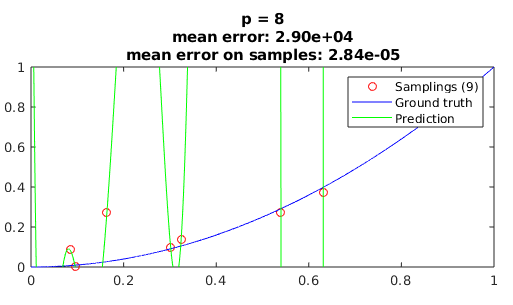
\includegraphics[width=0.75\textwidth]{plots/regression/maximum_p.png}
\end{figure}

\subsubsection{$p<n-1$}

Per bassi valori di p, la funzione risultante é semplice. \\
Tra i vari valori di p, in questa particolare istanza,
il valore che approssima meglio la funzione originale é $p=4$
per il quale si ha il piú basso errore medio. \\
Questo significa che per questa funzione,
l'errore di approssimazione é inferiore a quello di stima. \\
Colpisce anche che il miglior stimatore non coincida con il grado della funzione originaria,
ció é dovuto al rumore. \\

\begin{figure}[H]
  \centering
  \begin{subfigure}{0.45\textwidth}
    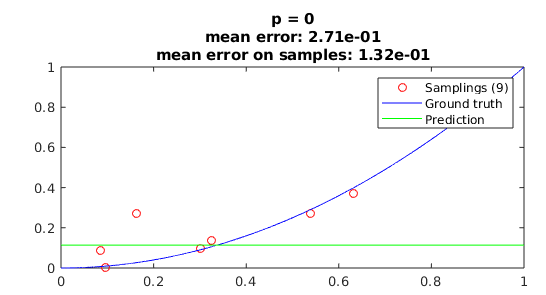
\includegraphics[width=\textwidth]{plots/regression/p_eq_0.png}
  \end{subfigure}
  \begin{subfigure}{0.45\textwidth}
    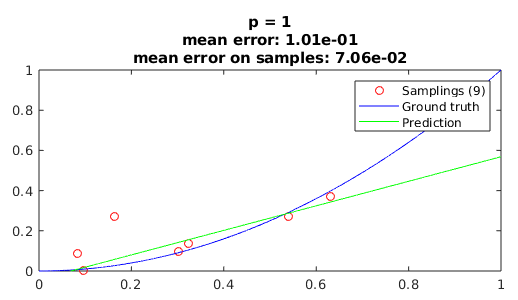
\includegraphics[width=\textwidth]{plots/regression/p_eq_1.png}
  \end{subfigure}
\end{figure}

\begin{figure}[H]
  \centering
  \begin{subfigure}{0.45\textwidth}
    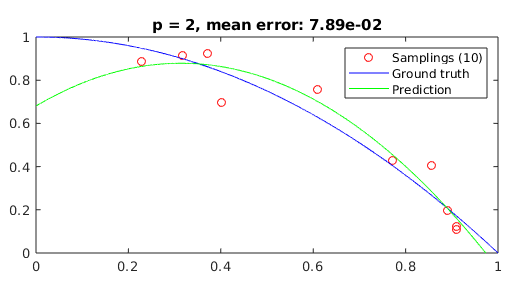
\includegraphics[width=\textwidth]{plots/regression/p_eq_2.png}
  \end{subfigure}
  \begin{subfigure}{0.45\textwidth}
    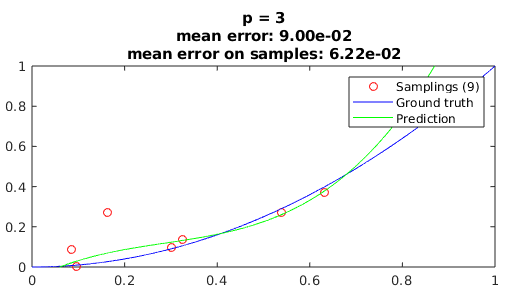
\includegraphics[width=\textwidth]{plots/regression/p_eq_3.png}
  \end{subfigure}
\end{figure}

\begin{figure}[H]
  \centering
  \begin{subfigure}{0.45\textwidth}
    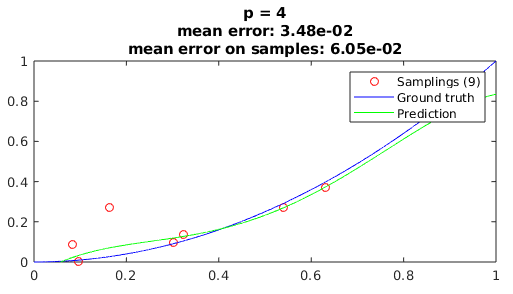
\includegraphics[width=\textwidth]{plots/regression/p_eq_4.png}
  \end{subfigure}
  \begin{subfigure}{0.45\textwidth}
    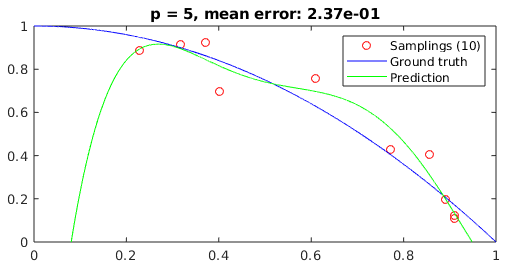
\includegraphics[width=\textwidth]{plots/regression/p_eq_5.png}
  \end{subfigure}
\end{figure}

\begin{figure}[H]
  \centering
  \begin{subfigure}{0.45\textwidth}
    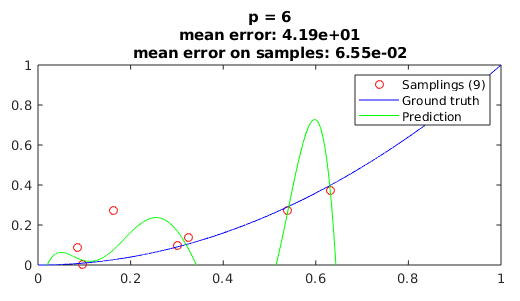
\includegraphics[width=\textwidth]{plots/regression/p_eq_6.png}
  \end{subfigure}
  \begin{subfigure}{0.45\textwidth}
    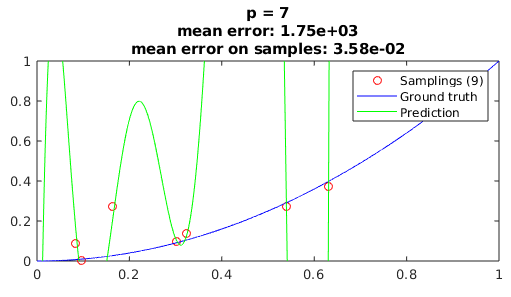
\includegraphics[width=\textwidth]{plots/regression/p_eq_7.png}
  \end{subfigure}
\end{figure}

\newpage
\subsection{Codice}
\lstinputlisting[basicstyle=\tiny ,language=MATLAB]{regressione.m}

\newpage
\section{Analisi di regressione in presenza del regolarizzatore}

\subsection{Introduzione}

Per questa analisi si introduce un nuovo parametro $\lambda$ detto \textit{regolarizzatore} \\
La funzione da minimizzare diviene

$$
  \underset{\underline{c}}{\min} \mid \mid X \underline{c} - \underline{y} \mid \mid^2 + \lambda \mid \mid \underline{c} \mid \mid^2
$$
Portando il calcolo di $ \underline{c} $ a:
$$
  \underline{c} = (X^T X + \lambda I)^+ X \underline{y}
$$
Il valore introdotto ha la funzione equivalente a un filtro low pass:
i termini di grado piú alto vengono smorzati, "ammorbidendo" la funzione risultante. \\
$\lambda \mid \mid \underline{c} \mid \mid$ rappresenta circa il numero di funzioni all'interno dello spazio delle ipotesi \\
e affinché questo valore sia convesso, viene elevato al quadrato.

\subsection{Parametri di simulazione}

Dimensione dell'asse delle x: $10000$ punti \\
Intervallo dell'asse delle x: $0 \leq x \leq 1$ \\
Punti campione: $10$ \\
Intensitá di rumore: $10\%$

\subsection{Analisi al variare di $\lambda$}

Per valori piccoli di $\lambda$ si ha overfit (in zero si ha che la funzione attraversa esattamente tutti i punti campionati). \\
Con il crescere di $\lambda$, la struttura della funzione ricostruita si semplifica (i coefficienti associati ai termini piú alti in grado risultano smorzati). \\
Per valori di $\lambda$ troppo elevati, la funzione diverge dai dati, tendendo a "appiattirsi".

Il valore di $\lambda$ che fornisce il minor errore rispetto alla funzione reale nel caso
considerato é $\lambda=1*10^{-2}$. \\
Non é possibile trarre una legge generale che associ l'errore medio al variare di $\lambda$.
Per quanto riguarda l'errore medio rispetto ai campioni, valori di lambda inferiori sono associati
a una maggiore vicinanza ai punti campionati, infatti per il caso limite $\lambda=0$ si ha una funzione che
attraversa esattamente tutti i punti utilizzati per la sua costruzione.

\begin{figure}[H]
  \centering
  \begin{subfigure}{0.45\textwidth}
    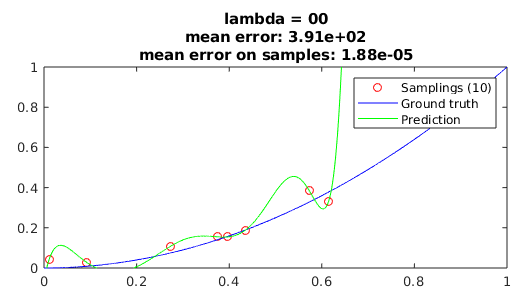
\includegraphics[width=\textwidth]{plots/regression_lambda/lambda_eq_0.png}
  \end{subfigure}
  \begin{subfigure}{0.45\textwidth}
    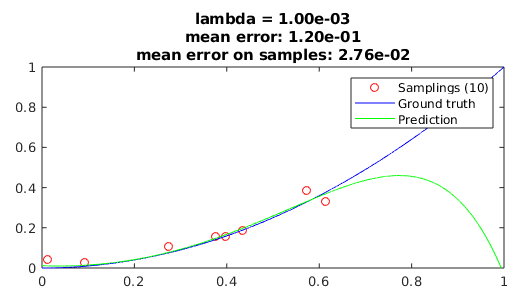
\includegraphics[width=\textwidth]{plots/regression_lambda/lambda_eq_10-3.png}
  \end{subfigure}
\end{figure}

\begin{figure}[H]
  \centering
  \begin{subfigure}{0.45\textwidth}
    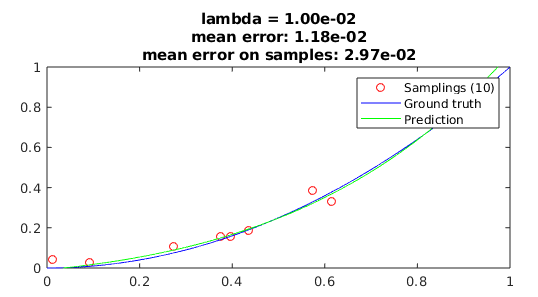
\includegraphics[width=\textwidth]{plots/regression_lambda/lambda_eq_10-2.png}
  \end{subfigure}
  \begin{subfigure}{0.45\textwidth}
    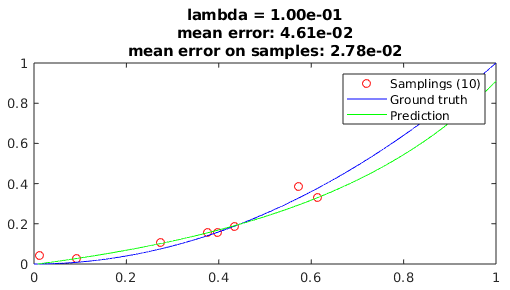
\includegraphics[width=\textwidth]{plots/regression_lambda/lambda_eq_10-1.png}
  \end{subfigure}
\end{figure}

\begin{figure}[H]
  \centering
  \begin{subfigure}{0.45\textwidth}
    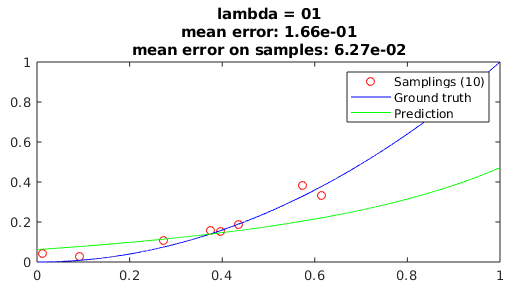
\includegraphics[width=\textwidth]{plots/regression_lambda/lambda_eq_1.png}
  \end{subfigure}
  \begin{subfigure}{0.45\textwidth}
    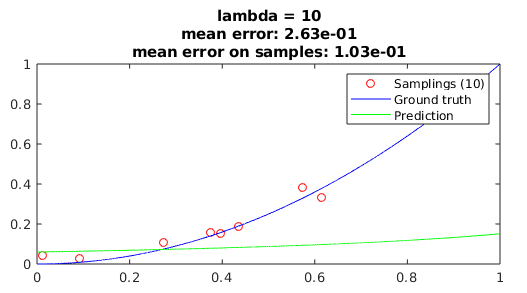
\includegraphics[width=\textwidth]{plots/regression_lambda/lambda_eq_10.png}
  \end{subfigure}
\end{figure}

\newpage
\subsection{Codice}
\lstinputlisting[basicstyle=\tiny ,language=MATLAB]{regressione_lambda.m}

\newpage
\section{Analisi di Monte Carlo dei due approcci}

\subsection{Parametri}

Numero di trials: $1000$

\subsection{Regressione}

\begin{verbatim}
p = 0, error = 2.66e-01
p = 1, error = 7.90e-02
p = 2, error = 5.64e-02
p = 3, error = 9.54e-02
p = 4, error = 2.27e-01
p = 5, error = 1.10e+00
p = 6, error = 9.00e+00
p = 7, error = 1.37e+02
p = 8, error = 2.96e+03
\end{verbatim}

\subsubsection{Codice}
\lstinputlisting[basicstyle=\tiny ,language=MATLAB]{regressione_mc.m}

\newpage
\subsection{Regressione con regolarizzatore}

\begin{verbatim}
lambda = 0.00e+00, error = 1.00e+04
lambda = 1.00e-03, error = 3.69e-02
lambda = 1.00e-02, error = 2.94e-02
lambda = 3.16e-02, error = 2.80e-02
lambda = 1.00e-01, error = 3.11e-02
lambda = 3.16e-01, error = 4.39e-02
lambda = 1.00e+00, error = 6.99e-02
lambda = 3.16e+00, error = 1.11e-01
lambda = 1.00e+01, error = 1.65e-01
\end{verbatim}
Come precedentemente indicato, l'errore maggiore si commette per
$\lambda=0$. \\
Con la crescita di $\lambda$, dopo una certa soglia, l'errore incrementa monotonicamente.

\subsubsection{Codice}
\lstinputlisting[basicstyle=\tiny ,language=MATLAB]{regressione_lambda_mc.m}

\end{document}
